\begin{XeClass}{BlockLocation}
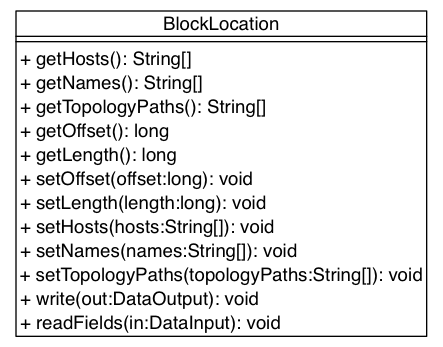
\includegraphics[width=10cm]{cdig/BlockLocation.png}
     
 \emph{BlockLocation}是块位置类.
 域包含主机号、端口号、拓扑路径以及偏移量和长度信息
 主要方法为域的get、set方法和实现Writable接口的读写方法

    \begin{XeMethod}{\XePublic}{String[]}{getHosts}
         
 获取主机名列表

    \end{XeMethod}

    \begin{XeMethod}{\XePublic}{String[]}{getNames}
         
 获取端口号列表

    \end{XeMethod}

    \begin{XeMethod}{\XePublic}{String[]}{getTopologyPaths}
         
 获取每一个主机的网络拓扑路径的列表,路径的最后部分是主机

    \end{XeMethod}

    \begin{XeMethod}{\XePublic}{long}{getOffset}
         
 获取块的偏移量

    \end{XeMethod}

    \begin{XeMethod}{\XePublic}{long}{getLength}
         
 获取块的长度信息

    \end{XeMethod}

    \begin{XeMethod}{\XePublic}{void}{setOffset}
         
 设置快的偏移量

    \end{XeMethod}

    \begin{XeMethod}{\XePublic}{void}{setLength}
         
 设置块的长度信息

    \end{XeMethod}

    \begin{XeMethod}{\XePublic}{void}{setHosts}
         
 设置当前块的主机名

    \end{XeMethod}

    \begin{XeMethod}{\XePublic}{void}{setNames}
         
 设置当前块的端口号

    \end{XeMethod}

    \begin{XeMethod}{\XePublic}{void}{setTopologyPaths}
         
 设置主机的网络拓扑路径

    \end{XeMethod}

    \begin{XeMethod}{\XePublic}{void}{write}
         
 实现Writable的write方法,主要是将块位置的
 各参数信息写到输出缓存中

    \end{XeMethod}

    \begin{XeMethod}{\XePublic}{void}{readFields}
         
 实现Writable的readFields方法
 读入块位置的各参数信息

    \end{XeMethod}

\end{XeClass}
